% ---------------------------------------------------------------------------
%  A Grammar-Driven Rule-Based Stemmer for Pashto
%
%  BUILD WITH XeLaTeX (or LuaLaTeX). Pashto is written in an extended Arabic
%  script, so a Unicode engine with a complex-script font is required;
%  pdflatex will not do.
%
%      xelatex main.tex && xelatex main.tex
%
%  The references are typeset with thebibliography, so no bibtex pass is
%  needed. Two passes resolve the cross-references.
%
%  Requirements:
%    * IEEEtran.cls   - TeX Live package texlive-publishers
%    * polyglossia, fontspec
%    * the font Noto Naskh Arabic. Substitute any installed Naskh font by
%      editing the \newfontfamily line below if it is not present.
% ---------------------------------------------------------------------------
\documentclass[conference]{IEEEtran}

\usepackage[T1]{fontenc}
\usepackage{booktabs}
\usepackage{longtable}
\usepackage{array}
\usepackage{graphicx}
\usepackage{amsmath}
\usepackage{url}
\usepackage[hidelinks]{hyperref}

% ---- Pashto (right-to-left, Arabic script) ----
\usepackage{fontspec}
\usepackage{polyglossia}
\setmainlanguage{english}
\setotherlanguage{pashto}
\newfontfamily\pashtofont[Script=Arabic]{Noto Naskh Arabic}
\newcommand{\ps}[1]{{\pashtofont\textpashto{#1}}}

\begin{document}

\title{A Grammar-Driven Rule-Based Stemmer for Pashto}

\author{\IEEEauthorblockN{Khairullah Ibrahim Khail}
\IEEEauthorblockA{Institute of Management Sciences\\
Peshawar, Pakistan\\
ibrahimkhil976@gmail.com}}

\maketitle

% ===========================================================================
\begin{abstract}
Pashto has roughly forty million speakers and very few text-processing tools.
The only stemmer published for the language applies nine affix rules without a
lexicon and without any means of choosing between competing analyses. We
present a rule-based Pashto stemmer built from an affix inventory of 117 rules
drawn from published grammars, in which every rule records its source, its
productivity, and whether it may be applied at all. Candidate stems are
generated separately from the decision of which candidate to keep, so a
shallower analysis can displace a deeper one. No machine learning is used.

Since no annotated set for Pashto stemming existed, we built two. A development
set of 2{,}912 word types and a held-out set of 500 types sampled from news text
were each annotated independently by three native-speaker Pashto educators, who
agreed on 96.88\% of stems ($\kappa = 0.969$). The held-out set was annotated
with its reference column empty and was not consulted while the system was
being developed. 499 of its 500 types fall within the stemming task and are the
denominator below; the remaining one needs a different word and is reported
apart.

On that set the proposed system reaches 71.34\% exact-match accuracy against
40.48\% for a faithful reimplementation of the prior system, and 70.6\% against
16.9\% on the types that carry an affix. Paice's under-stemming index falls
from 0.889 to 0.500.

A secondary finding concerns evaluation itself. The protocol used in the prior
work---presenting system output to native speakers and asking whether it is
acceptable---assigns a score of 100\% to a system that modifies no word at
all. We report results under both that protocol and exact match against a
reference fixed in advance, and recommend the latter for Pashto stemming.
\end{abstract}

\begin{IEEEkeywords}
Pashto, stemming, morphological analysis, rule-based methods, low-resource
languages, evaluation methodology, information retrieval
\end{IEEEkeywords}

% ===========================================================================
\section{Introduction}

A reader searching for documents about houses does not distinguish between
\emph{house}, \emph{houses} and \emph{of the houses}. A retrieval system does,
because to the system these are three unrelated strings. Stemming removes that
difference by stripping the endings a word carries, so that related forms
collapse onto a single index term. For English the problem has been settled
since Porter's algorithm~\cite{porter1980}, which remains in production use
after four decades.

For Pashto almost nothing exists. The language is spoken by approximately
forty million people across Afghanistan and Pakistan, is one of the two
official languages of Afghanistan, and has a growing volume of digital text in
news and social media. It also has a rich inflectional system, which is
precisely the condition under which stemming matters. A Pashto retrieval
system without stemming will miss most relevant documents; a classifier will
treat the singular and plural of a key term as unrelated features and learn
each from less data than it has.

The single published Pashto stemmer, by Aslamzai and Saad~\cite{aslamzai2015},
applies nine affix rules in a fixed order with no lexicon and no selection
stage. Our reimplementation of those rules leaves most words untouched, and
damages a substantial fraction of the words it does modify.

Three properties of Pashto make a naive approach fail.

\subsection{Five letters for one sound}

Pashto writes five distinct characters conventionally called \emph{ye}. They
are not interchangeable; they carry gender, number and case:

\begin{center}
\begin{tabular}{llp{4.4cm}}
\toprule
Letter & Example & Function\\
\midrule
\ps{ی} & \ps{سړی} & masculine singular direct\\
\ps{ي} & \ps{سړي} & masculine plural/oblique; 3rd person present\\
\ps{ې} & \ps{ښکلې} & feminine; plural\\
\ps{ۍ} & \ps{نجلۍ} & feminine singular, one noun class\\
\ps{ئ} & \ps{ووایئ} & 2nd person plural imperative\\
\bottomrule
\end{tabular}
\end{center}

Normalization pipelines written for Persian or Urdu routinely merge these into
a single character. For Pashto that destroys the information a stemmer needs:
\ps{سړی} (man) and \ps{سړي} (men) become indistinguishable. Our system
preserves all five.

\subsection{Endings that are not endings}

The same final letter may be an affix in one word and part of the root in
another, with nothing in the surface form to separate the two cases:
\ps{لنډه} reduces to \ps{لنډ}, where \ps{ه} marks agreement, while \ps{سیمه}
must remain \ps{سیمه}, because there the \ps{ه} belongs to the word. A native
speaker resolves this by knowing the word; a rule conditioned on the surface
form cannot.

\subsection{Verbs whose stems cannot be derived}

Pashto distinguishes weak verbs, whose stems follow from the infinitive, from
strong verbs, whose present stem must be known: \ps{لیدل} has the present stem
\ps{وین}, and \ps{تلل} has \ps{ځ}. No affix rule derives \ps{وین} from
\ps{لیدل}. These verbs are frequent and must be listed.

\subsection{Contributions}

\begin{itemize}
\item An affix inventory of 117 rules in which each entry records its
grammatical source, its productivity, a confidence level, and an explicit
decision about whether it may be stripped. Twenty-seven entries are documented
but never applied.
\item Two annotated evaluation sets for Pashto stemming, one of which was
annotated blind and never used during development.
\item An evaluation protocol that separates performance on word types carrying
an affix from performance on types that do not, because overall accuracy alone
rewards inactivity in a language where nearly half of word types are
uninflected.
\item A quantitative account of what each component contributes, including two
components that we retain despite a measured cost and one rule that we
implemented, measured and removed.
\item The observation that the evaluation protocol used in prior Pashto
stemming work cannot distinguish a working stemmer from an inert one.
\end{itemize}

% ===========================================================================
\section{Related Work}

\subsection{Rule-based stemming}

Lovins~\cite{lovins1968} published the first English stemmer, a single-pass
longest-match algorithm over 294 endings. Porter~\cite{porter1980} replaced it
with a five-step procedure whose conditions depend on a measure of syllable
count. Its durability is instructive: the algorithm is small, fast, entirely
inspectable, and makes no claim to produce real words. Porter maps both
\emph{relational} and \emph{relate} to \emph{relat}, which is not an English
word. The output of a stemmer is a class label rather than a lemma, and
confusing the two is a recurring error in work on morphologically rich
languages.

Paice~\cite{paice1990} contributed both an algorithm and, more consequentially
for the present work, an evaluation method~\cite{paice1994}. His
under-stemming index counts related word pairs a system fails to conflate, and
his over-stemming index counts unrelated pairs it wrongly merges. Because the
two move in opposite directions, reporting both is more informative than
accuracy alone.

\subsection{Arabic-script languages}

Khoja and Garside~\cite{khoja1999} built an Arabic root extractor that strips
affixes and matches the remainder against triliteral patterns. Larkey,
Ballesteros and Connell~\cite{larkey2002} showed that light stemming, removing
only a short list of prefixes and suffixes, outperforms aggressive root
extraction for retrieval. Their conclusion shaped the design adopted here:
removing less, but removing it reliably, is preferable to removing more. For
Persian, Sharifloo and Shamsfard~\cite{sharifloo2008} used a bottom-up parser
over a morpheme lexicon. The pattern common to these systems is that a lexicon
resolves ambiguity that rules alone cannot.

\subsection{Pashto}

Work on Pashto stemming is confined, to our knowledge, to Aslamzai and
Saad~\cite{aslamzai2015}. Because that system is the baseline for everything
reported here, we describe it in full.

Their algorithm applies nine rules, four removing suffixes and five removing
prefixes, each with a length condition. Rule~1 removes one of eleven suffixes
from words of five or more characters; Rule~2 replaces a final \ps{ي} with
\ps{ه} in words of four or more; Rule~3 removes \ps{من}; Rule~4 removes
\ps{یز} and appends \ps{ه}; Rules~5, 6, 7 and 9 remove prefixes; and Rule~8
reduces a reduplicated word to one copy.

Reproducing the baseline exactly mattered, since a comparison against a
misimplementation would be worthless. Our implementation reproduces all eight
worked examples given in the paper. Four points in the publication required a
decision, and we record them so that they can be checked:

\begin{itemize}
\item The order of prefix and suffix removal is not stated. We remove suffixes
first, because the paper's own example \ps{موتروان} $\rightarrow$ \ps{موتر}
only succeeds in that order; with prefixes first, the Rule~5 prefix \ps{م}
removes the first letter of \ps{موتر}.
\item Rule~3 is stated for words of ``more than 5 characters'' but its example
\ps{واکمن} has exactly five, so we implement the condition as five or more.
\item The Rule~5 prefix list contains a bare \ps{م}, which contradicts the
\ps{موتروان} example above. We exclude it, giving the baseline the reading its
own example implies rather than the one that would lower its score.
\item Rule~4 instructs the reader to remove \ps{یز} and append \ps{ه}. Its
first example follows this, but its second gives \ps{دودیز} $\rightarrow$
\ps{دود} with no \ps{ه}.
\end{itemize}

Rule~2 is also linguistically incorrect as published. It maps the masculine
plural adjective \ps{ښکلي} to \ps{ښکله}, which is the feminine singular;
Tegey and Robson~\cite{tegey1996} give the masculine singular \ps{ښکلی} as the
base form of this class. The rule is corrected in our inventory.

Finally, the reported accuracy of 87\% is not comparable with the figures in
this paper, and the difference lies in the protocol rather than in the
algorithm. We return to this in Section~\ref{sec:protocol}.

\subsection{Grammatical sources}

The affix inventory was assembled from published descriptions rather than by
inspecting a corpus. Table~\ref{tab:sources} lists the sources used and the
tag each carries in the released inventory file.

Of the 117 rules, 111 cite a published source, located by chapter in Tegey and
Robson~\cite{tegey1996} or by section in Penzl~\cite{penzl1955}. The remaining
six---\ps{ستان}، \ps{نی}، \ps{نۍ}، \ps{نې}، \ps{لو}، \ps{ل}---are entries
the engine never applies. For those no grammar is being appealed to: the affix
is real Pashto morphology, the reason it is recorded is that a reader would
otherwise wonder why it is absent, and the reason it is not applied is measured
behaviour, given with each entry in Appendix~A. Every rule the engine can
actually fire cites a published source.

The provenance of each rule is recorded in Appendix~A rather than summarised,
so a reader can check any individual entry. One distinction a single citation
count would hide is worth drawing: twenty-two of the cited rules are documented
and never applied. For those the citation establishes that the affix exists,
not that removing it is safe, and the decision not to strip rests on measured
behaviour rather than on the grammar.

\begin{table}[t]
\caption{Sources for the affix inventory.}
\label{tab:sources}
\centering
\begin{tabular}{p{4.4cm}l}
\toprule
Source & Tag\\
\midrule
Tegey \& Robson, \emph{A Reference Grammar of Pashto}~\cite{tegey1996} & [T\&R]\\
Robson \& Tegey, ``Pashto''~\cite{robson2009} & [R\&T]\\
David, \emph{Descriptive Grammar of Pashto}~\cite{david2014} & ---\\
Naeem \& Khan, derivational morphology~\cite{naeem} & [N\&K]\\
Khan, Pashto diminutives~\cite{khan2023} & [Khan23]\\
Penzl, \emph{A Grammar of Pashto}~\cite{penzl1955} & [Penzl]\\
Wiktionary / kaikki.org Pashto suffixes & [W]\\
\bottomrule
\end{tabular}
\end{table}

% ===========================================================================
\section{Pashto Morphology}

This section covers the parts of the morphology that bear on the design. It is
not a complete grammatical description.

\subsection{Orthography}

Beyond the Arabic inventory, Pashto adds retroflex and other consonants that
occur in neither Arabic nor Persian: \ps{ټ ډ ړ ږ ښ ځ څ ڼ ګ}. A word containing
any of these is certainly Pashto rather than a loan, and the system uses that
fact.

A complication became apparent only late in this work. The same suffix is
written with different \emph{ye} letters in different registers: dictionary
orthography prefers \ps{لومړی} where news orthography writes \ps{لومړي}. A
rule spelled in one convention does not fire on the other. The system
therefore compares a folded key when deciding whether a rule applies, while
the letters it writes out are never altered. Section~\ref{sec:results}
quantifies the effect.

\subsection{Nominal inflection}

Tegey and Robson divide Pashto nouns into masculine classes M1--M4 and
feminine classes F1--F3, each with its own plural and oblique endings. The
endings the system removes most often are \ps{ونه} and \ps{ونو} (masculine
plural and its oblique), \ps{ان} and \ps{انو} (animate plural and oblique),
\ps{ې} (feminine plural) and \ps{و} (oblique plural). Nominal inflection is
not a simple suffix-substitution system: gender, number, noun class and the
final shape of the stem can all trigger stem alternation.

\subsection{Verbal morphology}

Two productive patterns form verbs from nouns and adjectives. The
\ps{ېدل}~intransitive and \ps{ول}~transitive patterns are regular, so both are
handled by rule and neither appears in the dictionary:
\ps{جوړېدل}~$\rightarrow$~\ps{جوړ} and \ps{جوړول}~$\rightarrow$~\ps{جوړ}. For
strong verbs the present stem cannot be predicted, and these are listed:
\ps{لیدل}~/~\ps{وین}, \ps{تلل}~/~\ps{ځ}, \ps{کول}~/~\ps{کو},
\ps{غوښتل}~/~\ps{غواړ}.

\subsection{Loanwords}

Pashto has borrowed heavily from Arabic, Persian and English, and loanwords
are the principal remaining source of error, because their endings frequently
resemble Pashto affixes. The correct stem of \ps{منشي} is \ps{منشي}, not
\ps{منش}; of \ps{کورس} is \ps{کورس}, not \ps{کور}, which is a different word
meaning \emph{house}; and of \ps{بېجينګ} (Beijing) is the word itself, not
\ps{جينګ}. Arabic broken plurals are a related problem, formed by changing the
internal vowel pattern rather than by adding material, so that no suffix rule
can reach them.

% ===========================================================================
\section{Method}

Fig.~\ref{fig:pipeline} shows the order in which a word passes through the
system. Three of the stages can return a stem on their own, and the remaining
word goes to the generate-and-select stages that do the general work. Every
stage can be disabled independently, which is what makes the component study in
Section~\ref{sec:results} possible.

\begin{figure}[t]
\centering
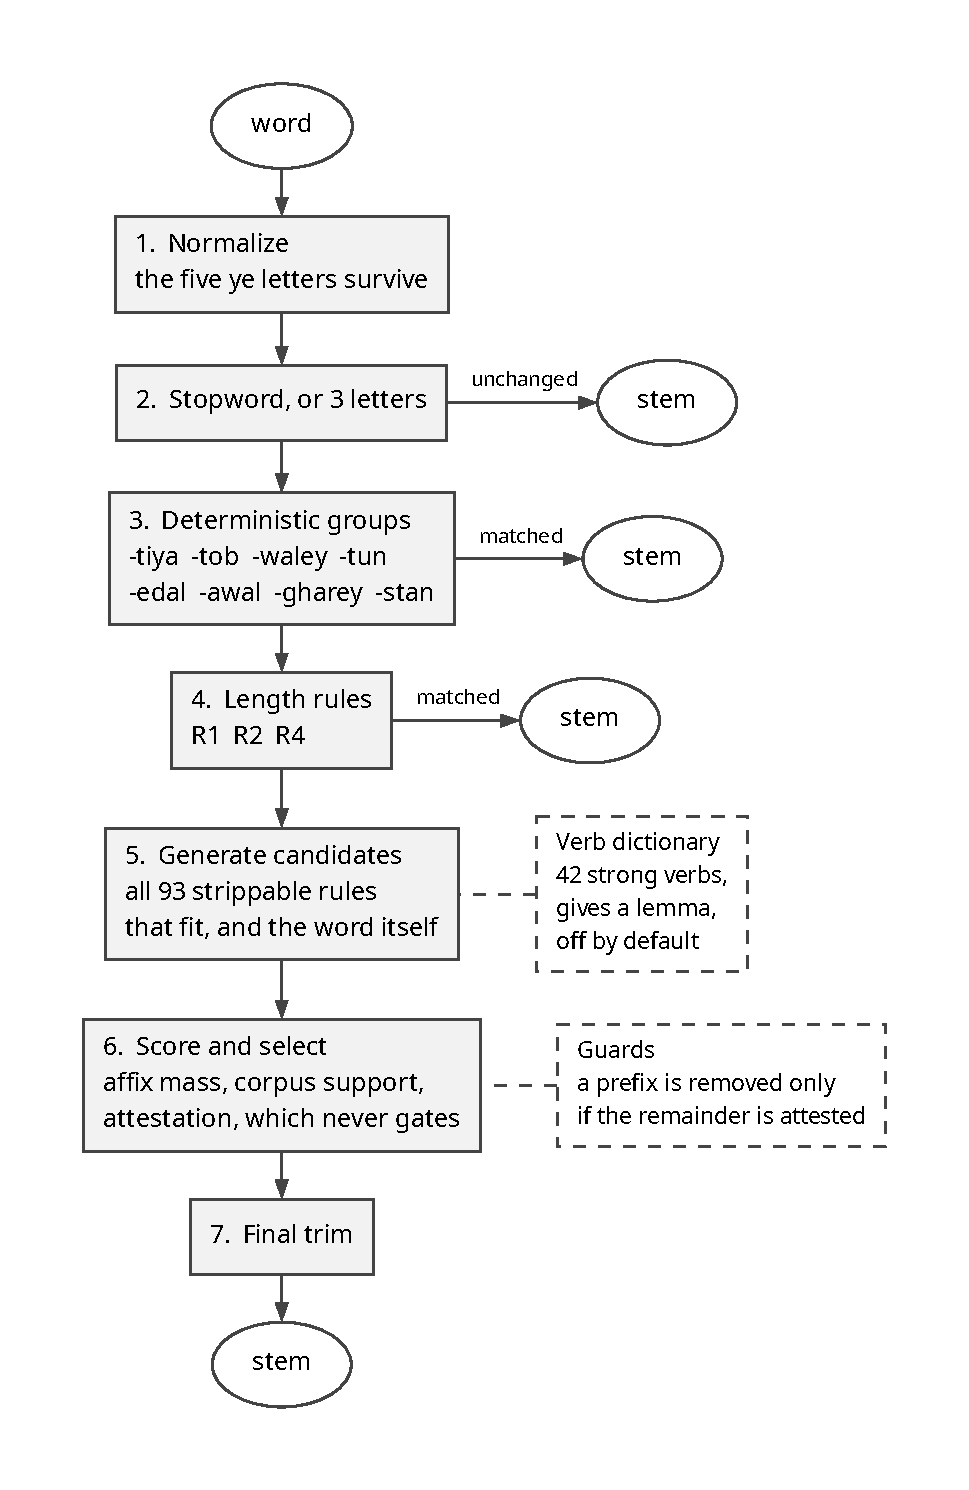
\includegraphics[width=\columnwidth]{figures/pipeline.pdf}
\caption{The pipeline. Stages 2--4 can each return a stem and stop; everything
else reaches stage 5, where all applicable rules are applied and the results
are then scored against one another. The two dashed boxes are not stages: the
guards constrain which strips the earlier stages may make, and the
irregular-verb dictionary is an optional lemmatization mode that is off by
default. Affixes are transliterated in the figure for legibility and given in
Pashto script in the text.}
\label{fig:pipeline}
\end{figure}

\subsection{Normalization}

Normalization removes differences that carry no information: Arabic
diacritics, the tatweel elongation character, zero-width joiners, and the
several Unicode encodings of the same letter. The Arabic kaf is mapped to the
Pashto keheh, the alef-hamza forms to bare alef, and the Urdu letters common
in Pashto written in Pakistan (\ps{ٹ ڈ ڑ ے} and the Persian \ps{گ}) to their
Pashto counterparts. These are encoding corrections rather than changes of
spelling.

What normalization does not do is merge the \emph{ye} letters. We verified
that no \emph{ye} character is altered in any cell of either evaluation set.
This holds through the whole pipeline, not only at the normalization step: the
output is always a slice of the input token, so whichever \emph{ye} the word
was written with is the one the stem carries. A rule spelled with \ps{ی} that
fires on a word spelled with \ps{ي} returns \ps{ي}.
The aggressive fold remains available behind a configuration flag so that the
cost of the error reported in the literature can be measured rather than
asserted.

\subsection{The affix inventory}

The inventory holds 107 suffix rules and 10 prefix rules. Each rule records
the affix and the side it attaches to; whether it is inflectional or
derivational; a minimum surviving stem length; the part of speech the affix
signals, where known; its productivity (productive, restricted, lexicalized or
borrowed); a confidence level; and whether it may be stripped at all.

Table~\ref{tab:schema} gives the schema in full, with three entries written
out. The last field does real work. Twenty-seven entries are documented but
never applied, because applying them was measured to be harmful or because the
grammatical source provides no attested example. The lexicalized diminutive
\ps{وکی}, the third column of Table~\ref{tab:schema}, is one: it survives only
in fixed words such as \ps{وړوکی}, so removing it by rule damages them.
Recording the affix and refusing to strip it is not the same as omitting it,
because the inventory is also a description of the language. The minimum stem
length does equally real work: without it the verb \ps{کېدل} reduces to the
single letter \ps{ک}.

\begin{table}[t]
\caption{The rule schema, with three entries written out. The third is
documented and never applied.}
\label{tab:schema}
\centering
\begin{tabular}{llll}
\toprule
Field & \ps{ونه} & \ps{توب} & \ps{وکی}\\
\midrule
side          & suffix        & suffix        & suffix\\
category      & inflectional  & derivational  & derivational\\
min.\ stem    & 2             & 3             & 3\\
POS signalled & N             & N             & N\\
productivity  & productive    & productive    & lexicalized\\
confidence    & high          & high          & low\\
strip allowed & yes           & yes           & \textbf{no}\\
source        & [T\&R] M2     & [N\&K]        & inventory \S4\\
\midrule
example       & \ps{کورونه}   & \ps{مینتوب}  & \ps{وړوکی}\\
              & $\rightarrow$ \ps{کور} & $\rightarrow$ \ps{مین}
              & unchanged\\
\bottomrule
\end{tabular}
\end{table}

Table~\ref{tab:inventory} groups the 117 rules by what they do. Derivation
accounts for 81 of them against 36 inflectional rules, which is the opposite of
what a stemmer for English would need and follows from where Pashto puts its
productive morphology. The grouping also shows where the gated entries are
concentrated: 17 of the 28 are noun-forming derivational suffixes, which is the
area where lexicalization is commonest and where a rule is most likely to be
documented in a grammar and still be unsafe to apply.

\begin{table}[t]
\caption{The 117 rules by function. ``Published'' counts the rules citing a
published grammar or lexical resource; ``kept'' counts those documented and
never stripped. The full inventory is Appendix~A.}
\label{tab:inventory}
\centering
% generated by paper/make_inventory_tables.py -- do not edit
\begin{tabular}{lcccl}
\toprule
Group & Rules & Published & Kept & Examples\\
\midrule
Nominal inflection & 23 & 23 & 0 & \ps{ونه انو ې}\\
Verbal inflection & 13 & 11 & 2 & \ps{ېدل ول}\\
Derivation: nouns & 56 & 54 & 17 & \ps{توب تیا تون}\\
Derivation: adjectives & 14 & 12 & 4 & \ps{یز مند ناک}\\
Derivation: verbs & 1 & 1 & 1 & ---\\
Prefixes & 10 & 10 & 4 & \ps{هم بیا نیم}\\
\midrule
Total & 117 & 111 & 28 & \\
\bottomrule
\end{tabular}

\end{table}

\subsection{Length rules}

Three rules were contributed by the author, a native speaker of Pashto, from
his own judgement, and then tested against the annotated data. A word of three letters or fewer
is returned unchanged. A word of four or five letters ending in one of the
five \emph{ye} letters or in \ps{ه} loses that letter. A word ending in
\ps{ستان} loses that suffix, and stripping stops there.

The last condition is necessary: allowing the general rules to continue
produced \ps{ترکمنستان}~$\rightarrow$~\ps{ترک} rather than \ps{ترکمن}. The
second rule originally included \ps{ل}, which we removed after measuring it.
On a verb \ps{ل} is the infinitive ending, but on a noun it is part of the
root, and the rule could not distinguish the two: it reduced \ps{کابل} to
\ps{کاب} and \ps{لامل} to \ps{لام}, accounting for 51 over-strips on its own.

A fourth rule was proposed and rejected. It would have removed the last three
characters of any non-Pashto word of seven characters or more. Measured against
three independent references, removing a documented affix instead was more
accurate in both careful annotations (45.0\% against 25.0\% on the development
set, 51.6\% against 43.5\% on the held-out set). Every word the rule damaged
carried a genuine affix: \ps{مسووليت} became \ps{مسوو} where the affix is
\ps{یت}, and \ps{اعلانات} became \ps{اعلا} where the affix is \ps{ات}. The
rule fired before the inventory was consulted and cut through the root.

\subsection{Candidate generation and selection}

Generation and selection are separate, which is the central design decision
borrowed from the Persian and Urdu hybrid systems. The generator applies every
rule that fits and returns all distinct forms reached, including the original
word with nothing removed. For \ps{کورونو} the pool contains the untouched
form, the result of removing \ps{ونو}, and the result of removing \ps{و}
alone. Nothing is decided at this stage, which is what allows a shallower
analysis to displace a deeper one.

A word that is already a stem is not passed through untouched by default. Below
the length rules it enters the same competition as any other word, as the
no-strip candidate, and it can lose: that is why the system modifies 68.3\% of
held-out types while the reference modifies 62.7\%, and why the
do-nothing floor is not a floor the system inherits.

Selection scores each candidate on how much affix material was removed,
whether other words in the corpus are built on the same stem, and whether the
stem itself is attested. For a candidate stem $c$ reached by removing $k$
characters, the score is

\begin{equation*}
v(c) = \beta k + F\!\cdot\![\,\mathrm{fam}(c) \ge 2\,] +
\begin{cases}
A_k + w_f\,\mathrm{freq}(c) & c \text{ attested}\\[2pt]
\gamma k & \text{otherwise}
\end{cases}
\end{equation*}

where $\mathrm{fam}(c)$ counts the distinct corpus words formed from $c$ by a
known suffix, $\mathrm{freq}(c)$ is the candidate's normalised corpus
frequency, and $A_k$ is the attestation bonus, which takes a smaller value when
$k=0$. Table~\ref{tab:weights} gives the constants. The family term fires only
when the remainder is at least three characters long.

\begin{table}[t]
\caption{Weights in the selection score. They were set by hand and adjusted on
the development set; none were fitted automatically, and the held-out set was
not used to choose any of them.}
\label{tab:weights}
\centering
\begin{tabular}{llr}
\toprule
Symbol & Meaning & Value\\
\midrule
$\beta$   & reward per character removed & 0.50\\
$F$       & bonus when the remainder has a word family & 2.00\\
$A_{k>0}$ & attestation bonus for a stripped candidate & 2.00\\
$A_{0}$   & attestation bonus for the unstripped word & 0.50\\
$w_f$     & weight on corpus frequency & 0.50\\
$\gamma$  & reward per character for an unattested strip & 0.20\\
\bottomrule
\end{tabular}
\end{table}

Two of these carry the design decisions. $A_0$ is a quarter of $A_{k>0}$
because the unstripped word is nearly always in the corpus, and giving it the
full bonus made inaction the default winner. And $\gamma>0$ is what lets the
rules act on a word the lexicon has never seen: an unattested strip still
scores above zero, so out-of-vocabulary input is stemmed rather than returned
whole, though it loses to any attested candidate. Two corrections to this stage were necessary during
development and are worth recording, since both are easy to get wrong.

First, an early version required the stem to be an attested Pashto word before
accepting a strip. That is incorrect: the output of a stemmer is a class label,
and Porter's \emph{relat} is not an English word either. Attestation now
raises a candidate's score without gating it, and the system freely produces
stems that are not words, including \ps{ښوون}, \ps{لوبغاړ} and \ps{پوهن}.

Second, the unstripped input word is almost always present in the corpus, so
awarding it the full attestation bonus made inaction the default winner and
concealed every single-letter inflection. Presence in a corpus is evidence
that a string is a word, not that it is a stem, and the no-strip candidate now
receives a much smaller bonus.

A small number of affix groups bypass the scorer entirely; we call these the
uniform-strip group, and it is the component measured under that name in
Table~\ref{tab:ablation}. The abstract-noun and place suffixes \ps{تیا},
\ps{توب}, \ps{والی} and \ps{تون} are long and
unambiguous, so no competing analysis exists for the scorer to weigh; leaving
them arbitrated meant that \ps{روغتیا} and \ps{پوهنتون} remained unchanged
because \ps{روغ} and \ps{پوهن} are absent from the lexicon.

\subsection{Throughput}

The system is a single pass of string operations over a 117-rule table, with no
model to load. On one core of a commodity laptop it stems roughly 6{,}800 word
types per second cold and 7{,}100 warm, measured over the development set. For
an indexing pipeline the stemmer is not the bottleneck.

\subsection{Guards}
\label{sec:guards}

Two guards were added after error analysis. A prefix is removed only when what
remains is itself an attested word. Without it the system strips \ps{لا} from
\ps{لانسیټ}, leaving \ps{نسیټ}, and from \ps{لاانتها}, leaving \ps{انتها};
with it, both words are returned whole. The guard is conservative in both
directions, since \ps{لاانتها} genuinely is \ps{لا}~+~\ps{انتها}, and we
accept the missed strip in exchange for not cutting into loanwords.

The second guard concerns the interaction between the prefix rules and the
length rules. A word of four or five letters that begins with a removable
prefix is passed to the full inventory instead of simply losing its last
letter. Only a prefix that may actually be removed counts: \ps{نا} is kept
rather than stripped, so \ps{ناوړه} is still handled by the length rule and
becomes \ps{ناوړ}, which is what the annotation gives.

A third component was implemented and then removed. A compound splitter
returned the head of a word it judged to be a compound, which conflicted with
the annotation policy's decision to keep compounds whole. Measured, it fired on
seven types across the two evaluation sets and was wrong on all seven, usually
because the ``head'' it returned was itself a suffix:
\ps{نړۍوال}~$\rightarrow$~\ps{وال} and \ps{پټرولیم}~$\rightarrow$~\ps{یم}.
Disabling it is worth 0.22 points on the development set and 0.20 on held-out
text. Splitting Pashto compounds reliably needs a lexicon of free forms that we
do not have, and guessing at the boundary was worse than leaving it alone.

\subsection{The verb dictionary and the scope of the task}
\label{sec:scope}

The system includes a dictionary of 38 strong verbs covering 315 surface
forms, of which 23 are checked against a printed grammar and 15 are marked
unverified. The dictionary maps an inflected form to its verb:
\ps{شو}~$\rightarrow$~\ps{کېدل}. That output is usually the infinitive---182
of the 315 forms come back as the infinitive and the remaining 133 as a stem,
because the \ps{ل} is then removed by a suffix rule---and an infinitive is a
lemma, so substituting
one word for another is lemmatization rather than stemming. On the word types whose reference is a truncation, the dictionary
changes the output on 69 of them and is right on 11, because it supplies the
wrong kind of answer; it costs 1.36 points on the development set and 0.80 on
held-out text.

The dictionary is therefore disabled by default and provided as an explicit
lemmatization mode. We report its contribution separately in
Section~\ref{sec:results} rather than folding it into the stemming result.

% ===========================================================================
\section{Data and Annotation}

No annotated set for Pashto stemming was available, so two were constructed.
The distinction between them determines how the results should be read.

\subsection{Corpus}

Word frequencies were taken from a corpus of Pashto news and general text
assembled from VOA Pashto, BBC Pashto and a topic-labelled collection,
totalling approximately 5.4 million tokens and 68{,}850 distinct word types.
The lexicon shipped with the system is a 5{,}443-type frequency list drawn from
this material.

Building a larger lexicon from the full corpus was attempted and made results
worse. The reason is instructive: a raw corpus contains inflected forms as
well as base forms, so with 48{,}000 types the attestation signal ceased to
mean ``this is a stem'' and began rewarding over-stripped forms that happened
to occur. The smaller list was better by being sparser.

\subsection{Development set}
\label{sec:devset}

2{,}912 word types were annotated independently by three native speakers of
Pashto before the rule inventory was settled: the author, the principal of a
Pashto-medium school, and a university teacher of the language. None of the
three saw another's work, and none saw any system output. The author then
adjudicated the disagreements and produced the released reference.

Two of the three passes are released as separate files, and the agreement
between them can therefore be recomputed rather than asserted. On the 2{,}725
types both annotated, they chose the same stem for 96.88\%, which is a Cohen's
$\kappa$~\cite{cohen1960} of 0.969. Reduced to the decision that matters most---whether the word
carries an affix at all---they agree on 98.24\%, $\kappa = 0.965$. The two
coefficients answer different questions. Chance agreement on the full stem
string is 0.001, because the label space is every substring of the word, so
there $\kappa$ adds little to the raw figure; on the binary decision chance
agreement is 0.503, and the $\kappa$ is doing real work. Both fall in the band
Landis and Koch~\cite{landis1977} describe as almost perfect agreement.

The disagreements are small in substance as well as in number. Of the 86 types
the two annotators stem differently, 84\% differ by one or two characters:
\ps{مرست} against \ps{مرس}, \ps{خون} against \ps{خو}. They are disagreements
about how deep to cut, not about which analysis applies. The adjudicated
reference stays close to both passes: 93.64\% identical to the school
principal's and 94.98\% to the university teacher's. Where it departs from
both, it follows the written annotation policy, and the 42 policy decisions
taken during the project are logged individually with their reasons.

One part of the construction is circular and we state it rather than leave it to
be found. 116 verb forms were revised for consistency with the verb analysis,
and 81 of those were changed to the reading the system itself produces, which is
3.0\% of the stemming types. That is a real dependency between the reference and
the system, it is confined to verbs, and it is why the held-out set rather than
this one is treated as the result.

\subsection{Held-out set}

500 word types were sampled at random from the news corpus under three
constraints: a frequency of at least five, to exclude typographical noise; a
length of at least three characters; and no overlap with the development set.
The sample was annotated by the same three native speakers, with the reference
field initially empty so that nothing anchored them to any system's output. All
three agreed on the result, and it is released as a single reference column. The
set was not consulted during development, and every figure reported for it comes
from a single run of the finished system.

The first pass was audited by comparing every removal against the affix
inventory. On the released first-pass file, 77 of 327 removals, 23.5\%, match no
documented affix: words such as \ps{مزاج} and \ps{حارث}, which carry no affix
at all, had been shortened. Thirty rows were revised in response, and the figure
falls to 58 of 313, or 18.5\%. The same audit on the development set leaves 120
of 1{,}370 removals, or 8.8\%, unaccounted for.

That audit procedure is reusable and we recommend it. For each annotated pair,
the material removed is compared against the affix inventory; a removal
matching no affix is either an annotation error or evidence that the inventory
is incomplete, and inspection separates the two. Applied to the development
set, the same procedure identified six affixes the inventory lacked.

We went through all 58 removals that the audit leaves unaccounted for in the
final held-out set, and the split is informative. Thirty-three of them take
material off one end of the word. Twenty-three of those are gaps in the
inventory rather than errors in the annotation, and most are variants of
affixes already held: the oblique infinitive \ps{ولو} beside \ps{ول}, the
oblique \ps{ګرو} beside \ps{ګر}, the feminine \ps{یزې} beside \ps{یزه}, the
past participle \ps{ېدلې} beside \ps{ېدل}. Two more are combinations the
engine cannot form because it strips one layer at a time: \ps{توبونو} is
\ps{توب}~+~\ps{ونو}, and both halves are in the inventory. Eight are genuine
annotation errors, and they cluster where one would expect---the English loans
\ps{ایمرجینګ} and \ps{ریسایکلنګ}, where \ps{نګ} is not a Pashto affix, the
personal name \ps{ضیالرحمان}, the place name \ps{پچیراګام}. Two are
ambiguous.

The remaining twenty-five take material off both ends at once, and all of them
are verbs: \ps{وښيي}~$\rightarrow$~\ps{ښي},
\ps{رارسېدو}~$\rightarrow$~\ps{رسېد}. The ending is in the inventory in
every case; the prefix is a perfective or directional particle, and those are
not held, for the reason Section~IV.A gives---measured against both sets they
were right between 13\% and 50\% of the time. These rows are therefore
neither annotation errors nor an oversight in the inventory but the cost of
that decision, stated here rather than left out of the count. An earlier
version of the audit script reported only one-ended removals and so did not
list them at all.

That the one-ended errors run three to one towards missing affixes rather than
bad annotation is the useful part: it says the reference is sounder than the
rule list, and it names the twenty-three entries that would close the gap. The
classified list is released with a verdict and a reason on every row.

\subsection{Annotation policy}

The policy the annotations follow is released with the data. Its main
provisions are that the output is a stem and need not be a word; that Arabic
broken plurals are handled by dictionary lookup rather than by rule; that
proper nouns receive no special treatment, so \ps{افغانستان} loses its
\ps{ستان} like any other word; that compounds are kept whole; and that where
two analyses are both defensible, the shallower is preferred.

% ===========================================================================
\section{Evaluation Protocol}
\label{sec:protocol}

\subsection{Why exact-match accuracy alone is insufficient}

The natural measure is the proportion of word types for which the system
produces the annotated stem. On its own it is misleading. Nearly half of
Pashto word types carry no affix and should be returned unchanged, so a system
that modifies nothing scores 47.77\% on the development set and 37.27\% on the
held-out set. Every letter a system declines to remove earns it credit.

Tuning against overall accuracy therefore drives a stemmer towards inactivity.
During this work an apparent improvement of nearly three points proved, on
inspection, to be exactly that: the system had become more conservative, losing
seven points on the word types requiring a strip while gaining twelve on those
requiring none.

All results below report three figures: accuracy on the types the annotation
strips, accuracy on the types it leaves unchanged, and overall accuracy. The
first cannot be obtained by inaction.

\subsection{The scope of the stemming task}

Stemming removes characters; it cannot insert them. Where the reference is an
Arabic broken plural or a suppletive form---\ps{اثارو}~$\rightarrow$~\ps{اثر},
\ps{نجونو}~$\rightarrow$~\ps{نجلۍ}---the answer is a lemma that no affix rule
can produce. Marking a truncating stemmer wrong on those types penalises it for
not being a lemmatizer.

We therefore score the two tasks separately. A type belongs to the stemming
task when the reference is a substring of the word, which is exactly the case
where it can be reached by removing material from one end or from both;
comparison is insensitive to which \emph{ye} letter is written, since that is a
difference of register and not an affix. By this criterion the development set
contributes 2{,}717 stemming types and 195 lemma types, and the held-out set
499 and 1. Of the 195, 155 are verb forms whose reference is an infinitive that
no truncation reaches, \ps{شوه}~$\rightarrow$~\ps{کېدل} and
\ps{وایی}~$\rightarrow$~\ps{ویل}; the remaining 40 are suppletive or
irregular nominals such as \ps{نجونو}~$\rightarrow$~\ps{نجلۍ} and Arabic
broken plurals. The boundary between the two tasks is therefore almost entirely
the strong verb. Results for the lemma types are
reported separately in Section~\ref{sec:results}.

\subsection{Two protocols compared}

Aslamzai and Saad report 87\% accuracy; our reimplementation of the same nine
rules reaches 40.48\% on held-out data. The difference is entirely
methodological, and the point is important enough to measure rather than
assert.

Protocol~A, used throughout this paper, fixes the reference before any system
output is seen and counts a result only if it matches exactly. Protocol~B
reproduces theirs: a judge is shown the output and decides whether it is an
acceptable analysis. We implement Protocol~B reproducibly by counting an output
as acceptable when nothing was removed that is not a documented affix, and by
treating an unchanged word as always acceptable, which is how a judge shown an
unchanged word would score it.

\begin{table}[t]
\caption{The same 499 held-out word types under both protocols. The final
column gives the proportion of types the system modifies at all.}
\label{tab:protocol}
\centering
\begin{tabular}{lccc}
\toprule
System & A: exact & B: judged & Modified\\
\midrule
Modifies nothing       & 37.27\% & \textbf{100.00\%} & 0.0\%\\
Aslamzai \& Saad~\cite{aslamzai2015} & 40.48\% & 80.76\% & 37.5\%\\
\textbf{Proposed}      & \textbf{71.34\%} & \textbf{98.60\%} & 68.3\%\\
\bottomrule
\end{tabular}
\end{table}

The first row of Table~\ref{tab:protocol} is the finding. Under Protocol~B a
system that modifies no word scores 100\%, because every unchanged word is
acceptable to a judge and it produces nothing else. The protocol cannot
separate a working stemmer from an inert one, and a figure obtained under it
cannot be compared with an exact-match figure.

Nothing here shows the published 87\% to be incorrect. It shows that the
measurement answers a different question. We note that the proposed system
also outperforms the baseline under Protocol~B, by 98.60\% to 80.76\%, so the
conclusion does not depend on the choice.

% ===========================================================================
\section{Results}
\label{sec:results}

\subsection{Held-out evaluation}

Table~\ref{tab:heldout} reports the held-out set, which is the primary result:
499 word types from news text, annotated with the reference field initially
empty and never used during development.

\begin{table}[t]
\caption{Held-out evaluation, 499 word types. ``Affixed'' and ``Bare'' are
accuracy on the types the annotation changes and leaves unchanged.}
\label{tab:heldout}
\centering
\begin{tabular}{lcccc}
\toprule
System & Accuracy & Affixed & Bare & UI\\
\midrule
Modifies nothing & 37.27\% & 0.0\% & 100.0\% & 1.000\\
Aslamzai \& Saad & 40.48\% & 16.9\% & 80.1\% & 0.889\\
\textbf{Proposed} & \textbf{71.34\%} & \textbf{70.6\%} & 72.6\% & \textbf{0.500}\\
\bottomrule
\end{tabular}
\end{table}

The two systems fail in opposite directions, and that is more informative than
the gap between them. Of the baseline's 297 held-out errors, 254---86\%---are
under-strips, and 163 are words it left untouched altogether; only 9\% are
over-strips. Of our 143, 51\% are over-strips and 44\% under-strips. The
baseline's problem is inaction, ours is excess, which is the trade a stemmer
has to make and the reason the two halves of the task are reported separately.

The proposed system improves on the baseline by 30.9 points overall. The
separation of the two halves is more informative than the overall figure: on
the types that require a strip the baseline reaches 16.9\% and the proposed
system 70.6\%, a factor of four. Paice's under-stemming index falls from 0.889
to 0.500, and over-stemming remains below $4\times10^{-5}$.

\subsection{Development set}

\begin{table}[t]
\caption{Development set, 2{,}717 stemming types.}
\label{tab:dev}
\centering
\begin{tabular}{lcccc}
\toprule
System & Accuracy & Affixed & Bare & UI\\
\midrule
Modifies nothing & 47.77\% & 0.0\% & 100.0\% & 1.000\\
Aslamzai \& Saad & 50.68\% & 12.2\% & 92.8\% & 0.919\\
\textbf{Proposed} & \textbf{80.35\%} & \textbf{78.6\%} & 82.2\% & \textbf{0.304}\\
\bottomrule
\end{tabular}
\end{table}

Table~\ref{tab:dev} reports the development set. The figure is higher than the
held-out result. The revisions described in Section~\ref{sec:devset} account
for 0.07 points of that gap, so the explanation lies elsewhere: it is
orthographic, and Section~\ref{sec:orth} gives it. The development set is
reported for comparability with the baseline, which is scored identically, and
because Paice's indices are more stable on the larger set. On the types requiring a strip the margin is wider still: 78.6\%
against 12.2\%, a factor of six.

\subsection{Two external datasets}
\label{sec:external}

After the system was finalised, it was run against two independently annotated
Pashto word lists of 5{,}000 and 10{,}000 types. Neither was produced by this
project, and 96\% of their entries appear in neither of our evaluation sets.
Exact-match accuracy is 72.18\% and 70.15\% (Table~\ref{tab:external}), against
51.24\% and 47.95\% for the baseline. Those figures sit beside the 71.34\% measured on held-out news text,
which is the point: the system does not depend on the data it was built
against.

\begin{table}[t]
\caption{Two independently annotated word lists. The folded column compares
with the five \emph{ye} letters treated as equal; the stemmer's output is never
rewritten.}
\label{tab:external}
\centering
\begin{tabular}{lccc}
\toprule
Dataset & Types & Exact & Folded\\
\midrule
External, 5{,}000 types & 5{,}000 & 72.18\% & 80.28\%\\
\quad Aslamzai \& Saad & & 51.24\% & 57.36\%\\
External, 10{,}000 types & 10{,}000 & 70.15\% & 77.34\%\\
\quad Aslamzai \& Saad & & 47.95\% & 53.68\%\\
\midrule
Our held-out set & 499 & 71.34\% & 72.14\%\\
Our development set & 2{,}717 & 80.35\% & 81.85\%\\
\bottomrule
\end{tabular}
\end{table}

Both lists carry a reference column normalised to \ps{ی} while their word column
retains \ps{ي}, so a stem is scored wrong whenever it preserves the letter the
word actually has. Folding the five \emph{ye} letters together for the
comparison alone raises the two figures to 80.28\% and 77.34\%. The same folded
comparison is worth 1.51 points on our development set and 0.80 on our held-out
set, both of which are internally consistent in their orthography. The size of
that difference is what the measurement shows: seven to eight points on the
external lists against one on ours places the disagreement in how they spell the
reference rather than in the stemming.

One caveat limits what these lists establish. On the words they share with our
development set the two references agree 70.8\% and 64.1\% of the time. Sorting
the disagreements shows they are a difference of policy rather than noise.
About a quarter---19.1\% on the 5{,}000-type list and 24.3\% on the larger
one---are cases where our reference gives a lemma that no truncation reaches,
\ps{اخلی}~$\rightarrow$~\ps{اخیستل} against their \ps{اخ}; those are not
disagreements about stemming at all but about where stemming stops. Of the
rest, roughly half cut deeper than we do (\ps{تنګی}~$\rightarrow$~\ps{تن}
against our \ps{تنګ}) and about a quarter cut less
(\ps{استازیتوب}~$\rightarrow$~\ps{استازی} against our \ps{استاز}). Only two
disagreements in 154 come down to the spelling of a \emph{ye}. The two
annotations differ consistently in how deep a stem should go and in whether
verbs are reduced to a stem or to an infinitive, which is why these lists test
generalisation rather than correctness under our policy.

\subsection{Component study}

\begin{table}[t]
\caption{Each component removed in turn. Changes in percentage points.}
\label{tab:ablation}
\centering
\begin{tabular}{lcc}
\toprule
Configuration & Development & Held-out\\
\midrule
\textbf{Full system} & \textbf{80.35\%} & \textbf{71.34\%}\\
$-$ suffix rules & 71.99\% ($-$8.35) & 58.92\% ($-$12.42)\\
$-$ length rules & 77.70\% ($-$2.65) & 69.34\% ($-$2.00)\\
$-$ corpus lexicon & 80.16\% ($-$0.18) & 71.74\% ($+$0.40)\\
$-$ uniform-strip group & 80.13\% ($-$0.22) & 71.14\% ($-$0.20)\\
$-$ prefix rules & 80.31\% ($-$0.04) & 71.54\% ($+$0.20)\\
$+$ verb dictionary & 78.98\% ($-$1.36) & 70.54\% ($-$0.80)\\
\bottomrule
\end{tabular}
\end{table}

The suffix inventory does most of the work, and removing it costs 12.4 points
on held-out text. The author's length rules contribute between two and three
points on both sets.

Three rows record decisions taken against the measured score, and we state
them explicitly rather than quietly adopting whichever setting scored best.

Prefix stripping costs a few hundredths of a point on the development set. We
retain it because \ps{هم}, \ps{بیا}, \ps{نیم} and \ps{لا} are genuine Pashto
prefixes, and removing the rules would amount to claiming the language has
none; the attestation guard described in Section~\ref{sec:guards} is what
makes them safe. The small effect is itself explained by the inventory: of the
ten prefix rules, four are documented and never stripped. \ps{نا}, \ps{بې} and
\ps{غیر} are negation prefixes that the annotation policy keeps, because
\ps{ناقانونه} is not an instance of \ps{قانون} but its opposite, and \ps{سر}
is a free noun as often as it is a prefix.

The corpus lexicon is worth 0.18 points on the development set and $-0.40$ on
held-out text. Its contribution is now marginal, because the uniform-strip and
length rules decide most cases before the scorer is consulted. We report this
plainly: the system should not be described as lexicon-driven.

Enabling the verb dictionary costs 1.36 points on the development set and 0.80
on held-out text, for the reason
given in Section~\ref{sec:scope}. Its proper contribution is to the lemma
types, where it answers 51 of the 195 in the development set against 8 without
it.

\subsection{Orthography}
\label{sec:orth}

The gap between the two evaluation sets has one dominant cause. Of the 500
held-out news types, 118 contain the hard \emph{ye} \ps{ي}; of the 2{,}912
development types, none do. The inventory contained thirteen rules ending in
the narrow \emph{ye} \ps{ی} and none ending in \ps{ي}, so a large class of news
words passed through untouched: \ps{لومړي} and \ps{تاریخي} were returned
unchanged.

Making rule matching insensitive to which \emph{ye} is written, while leaving
the output letters untouched, corrected this. On the development set, which is
written entirely in one convention, exact matching scores 0.15 points higher;
on held-out news text the folded comparison is worth 1.20 points, so it earns
its place on the set that reflects real text. This is the clearest instance in
the project of a defect that a single-source evaluation set could not have
revealed.

% ===========================================================================
\section{Discussion}

\subsection{Correct rules and under-determined rules}

A per-rule analysis separates two kinds of failure, and the distinction matters
for how the remaining error should be addressed.

Table~\ref{tab:ruleprec} gives the precision of the rules that fire most often
on the development set: how many times each contributed to the analysis finally
selected, and how often that analysis matched the reference. Publishing it is
uncomfortable and necessary. A rule can contribute positive points overall and
still be wrong half the time it fires, and a reader cannot tell the two apart
from an ablation table.

\begin{table}[t]
\caption{Precision of the fourteen most frequently firing rules on the
development set. ``Fires'' counts the analyses finally selected in which the
rule took part. Generated by \texttt{experiments/error\_analysis.py}.}
\label{tab:ruleprec}
\centering
\begin{tabular}{lrrr}
\toprule
Rule & Fires & Correct & Precision\\
\midrule
R2 keep short word        & 398 & 357 & 89.7\%\\
R1 drop \ps{ه}            & 228 & 161 & 70.6\%\\
R1 drop \ps{ی}            & 190 & 149 & 78.4\%\\
R1 drop \ps{ې}            & 160 & 133 & 83.1\%\\
final trim                & 131 &  81 & 61.8\%\\
$-$\ps{ۍ}                 & 126 & 106 & 84.1\%\\
$-$\ps{و}                 & 108 &  88 & 81.5\%\\
$-$\ps{ونو}               &  58 &  54 & 93.1\%\\
R2 drop \ps{ې} at 3 letters&  39 &  21 & 53.8\%\\
$-$\ps{ونه}               &  39 &  35 & 89.7\%\\
$-$\ps{ه}                 &  36 &  24 & 66.7\%\\
R1 drop \ps{ۍ}            &  36 &  31 & 86.1\%\\
R2 drop \ps{و} at 3 letters&  32 &  18 & 56.2\%\\
$-$\ps{ان}                &  28 &  13 & 46.4\%\\
\bottomrule
\end{tabular}
\end{table}

Building that table changed the system. Two rules turned out to fire 26 times
between them and be right on none of those occasions: \ps{لو}, the oblique
infinitive, and \ps{لې}, the feminine past participle. Both bundle an \ps{ل}
into the affix that the reference keeps, either as the infinitive marker
(\ps{ساتلو}~$\rightarrow$~\ps{ساتل}, not \ps{سات}) or as part of the root
(\ps{بریالی}~$\rightarrow$~\ps{بریال}). The rules that remove the final vowel
alone already produce the right answer, so these two could only ever take one
letter too many. They are now documented and never applied, which is worth 0.85
points on the development set and nothing either way on held-out text. This is
the same defect as the standalone verbal \ps{ل}, which was removed earlier for
the same reason: it applied only to nouns where \ps{ل} belongs to the root and
turned \ps{کابل} into \ps{کاب}. Two further rules were removed during the work,
one taking \ps{نی} as a unit where the affix is usually the \ps{ی} alone, and
one restoring a feminine \ps{ه} to any stem that had lost one, which produced
\ps{کورونو}~$\rightarrow$~\ps{کورونه}.

Three rules remain below 60\% precision and are kept. \ps{ان} is right 13 times
in 28, but it is the ordinary animate plural of Pashto and gating it costs 0.40
points on held-out text; its low precision reflects competition with longer
analyses rather than a defect in the rule. The two three-letter length rules sit
at 53.8\% and 56.2\% for the reason the next paragraph describes, and the
alternative to a coin-flip there is to leave every short inflected word
unstemmed.

Other rules are correct but under-determined. The rule removing a final \ps{ه}
from a short word fires 228 times on the development set and is correct 161 of
those. \ps{لنډه}~$\rightarrow$~\ps{لنډ} is right and
\ps{خواړه}~$\rightarrow$~\ps{خواړ} is wrong, and the two words are
indistinguishable in shape. Removing the rule loses more than it saves: overall
accuracy falls by 1.62 points. No reformulation conditioned on the surface form
can help; only a lexical resource can.

\subsection{What limits the current accuracy}

The 534 development-set errors divide into three kinds. 291 of them, 54\%, are
over-strips, where the system removed more than the reference does; 202, 38\%,
are under-strips, and 102 of those are words the system left untouched
altogether; the remaining 41 are the same length as the reference but differ in
which letters survive. The held-out set behaves the same way, 51\% and 44\%.
Over-stripping is therefore the larger problem on both sets, which is what one
would expect of a system whose scorer rewards removing affix material.

Table~\ref{tab:bygroup} locates the errors. Each type is assigned to the group
of the rule that explains the reference's removal, under the same grouping as
Table~\ref{tab:inventory}, so that the two tables can be read against each
other. Accuracy is high wherever the reference removes an affix the inventory
holds---86.4\% on nominal inflection, 89.6\% on noun-forming derivation,
95.1\% on verbal inflection---and the two weak rows are the ones that do not
depend on the inventory being right. 120 types have a reference the inventory
cannot explain at all, and we reach 26.7\% on those. The larger group is the
1{,}347 types the reference leaves whole, where we are right 79.2\% of the
time: 280 words stripped that should not have been, the biggest single source
of error in the system.

\begin{table}[t]
\caption{Accuracy by the affix the reference removes, development set. The
grouping is the one in Table~\ref{tab:inventory}. Generated by
\texttt{experiments/error\_analysis.py}.}
\label{tab:bygroup}
\centering
\begin{tabular}{lrr}
\toprule
What the reference removes & Types & Accuracy\\
\midrule
Nominal inflection        & 1{,}116 & 86.4\%\\
Verbal inflection         &    41 & 95.1\%\\
Derivation: nouns         &    67 & 89.6\%\\
Derivation: adjectives    &    26 & 80.8\%\\
No affix, word left whole & 1{,}347 & 79.2\%\\
Nothing in the inventory  &   120 & 26.7\%\\
\bottomrule
\end{tabular}
\end{table}

We had attributed that bucket to loanwords, and the data does not support it.
Pashto marks native vocabulary orthographically: a word containing one of
\ps{ټ ډ ړ ږ ښ ځ څ ڼ ګ ې ۍ} is certainly not a borrowing, though a word without
one may be either, so the test is one-sided. Among the types the reference
leaves whole we are wrong on 28.3\% of the certainly-native ones and 17.6\% of
the rest. Native words are the harder half, not the easier one, and the errors
bear it out: \ps{خواړه}, \ps{وړاندې}, \ps{داسې}, \ps{پاتې}, \ps{یوازې} and
\ps{پورې} are ordinary Pashto words ending in \ps{ه} or \ps{ې} that the length
rules cut. The shortfall is the \ps{ه}/\ps{ی}/\ps{ې} ambiguity, and it falls on
native vocabulary rather than on borrowings.

We tested the obvious remedy and report the result because it is negative. A
257-entry list of development-set words that should be left unchanged raises
development accuracy by 8.5 points and held-out accuracy by zero: of the 51
held-out types needing the same treatment, none appear in the list. The list is
pure memorisation of one sample. The generalizing form of the same idea is a
lexicon of words that must not be stripped. On the evidence above it would need
to cover ordinary native vocabulary rather than borrowings alone, which makes
it a larger undertaking than we first assumed, and we leave it to future
work.

% ===========================================================================
\section{Limitations}

The evaluation is on word types rather than running text, so no measurement of
retrieval effectiveness is reported, and the relationship between the intrinsic
gains shown here and downstream performance remains untested.

Of 117 affix rules, 111 cite a published grammar by chapter or section; the
six that do not are entries the engine never applies. The chapter attributions
were assembled by the author and have not been independently checked page by
page, so a reader verifying the inventory should treat each locus as a pointer
rather than as a quotation. Of 38 verbs in the dictionary, 23 are checked against a
printed grammar and 15 are marked unverified in the released documentation. We
prefer to label these rather than to present them as settled.

Compounds are kept whole, which is a policy choice rather than a solution: it
avoids a class of error at the cost of never conflating \ps{لاسلیک} with
\ps{لاس}. The annotation does not follow the policy perfectly either, and an
audit during development found types where the reference itself splits a
compound. The released audit script
reports every removal that matches no documented affix, which is where such
cases surface.

The corpus is drawn from news and general text, so the vocabulary of
specialised domains is under-represented.

% ===========================================================================
\section{Conclusion}

We presented a rule-based stemmer for Pashto built from an affix inventory of
117 rules taken from published grammars, each recording its source, its
productivity and an explicit decision about whether it may be applied. No
machine learning is used, and every decision the system makes can be traced to
a rule or a dictionary entry.

On 499 held-out word types from news text, annotated blind and never used
during development, the system reaches 71.34\% exact-match accuracy against
40.48\% for the published baseline, and 70.6\% against 16.9\% on the types
that require a strip. On a 2{,}717-type development set it reaches 80.35\%
against 50.68\%, with Paice's under-stemming index falling from 0.919 to
0.304.

Three observations generalise beyond this particular system. Exact-match
accuracy is not a sufficient measure for stemming in a language where a large
share of word types carry no affix, because it rewards inactivity; reporting
the two halves of the task separately costs nothing and prevents the error. An
evaluation set drawn from a single orthographic convention will conceal defects
that a second source exposes immediately, as the \emph{ye} variants did here.
And when a rule-based system finds no affix, the useful response is to ask what
the inventory is missing rather than to remove characters regardless: the one
rule in this work that guessed a boundary instead of finding one was measured
against three references, lost on both careful annotations, and was removed.

The stemmer, the affix inventory with its sources, the verb dictionary, both
annotated sets and the scripts that reproduce every figure in this paper are
released under an MIT licence at
\url{https://github.com/Khairullah-Ibrahim-Khail/Pashto_Stemmer}. Every table
in this paper is regenerated by \texttt{experiments/reproduce\_paper.py}, and
the inter-annotator figures by \texttt{experiments/agreement.py}.

% ===========================================================================
\section*{Acknowledgment}

The author thanks the two native speakers who annotated the data alongside him:
the principal of a Pashto-medium school and a university teacher of Pashto.

\begin{thebibliography}{99}

\bibitem{aslamzai2015}
S. Aslamzai and S. Saad, ``Pashto language stemming algorithm,''
\emph{Asia-Pacific Journal of Information Technology and Multimedia},
vol.~4, no.~1, pp.~25--37, 2015.

\bibitem{porter1980}
M.~F. Porter, ``An algorithm for suffix stripping,''
\emph{Program}, vol.~14, no.~3, pp.~130--137, 1980.

\bibitem{lovins1968}
J.~B. Lovins, ``Development of a stemming algorithm,''
\emph{Mechanical Translation and Computational Linguistics}, vol.~11,
pp.~22--31, 1968.

\bibitem{paice1990}
C.~D. Paice, ``Another stemmer,'' \emph{ACM SIGIR Forum}, vol.~24, no.~3,
pp.~56--61, 1990.

\bibitem{paice1994}
C.~D. Paice, ``An evaluation method for stemming algorithms,'' in
\emph{Proc. 17th Annual International ACM SIGIR Conference}, 1994,
pp.~42--50.

\bibitem{khoja1999}
S. Khoja and R. Garside, ``Stemming Arabic text,'' Computing Department,
Lancaster University, Tech. Rep., 1999.

\bibitem{larkey2002}
L.~S. Larkey, L. Ballesteros, and M.~E. Connell, ``Improving stemming for
Arabic information retrieval: light stemming and co-occurrence analysis,''
in \emph{Proc. 25th Annual International ACM SIGIR Conference}, 2002,
pp.~275--282.

\bibitem{sharifloo2008}
A.~A. Sharifloo and M. Shamsfard, ``A bottom up approach to Persian
stemming,'' in \emph{Proc. 3rd International Joint Conference on Natural
Language Processing}, 2008.

\bibitem{tegey1996}
H. Tegey and B. Robson, \emph{A Reference Grammar of Pashto}.
Washington, DC: Center for Applied Linguistics, 1996.

\bibitem{robson2009}
B. Robson and H. Tegey, ``Pashto,'' in \emph{The Iranian Languages},
G. Windfuhr, Ed. London: Routledge, 2009.

\bibitem{david2014}
A.~B. David, \emph{Descriptive Grammar of Pashto and its Dialects}.
Berlin: De Gruyter Mouton, 2014.

\bibitem{penzl1955}
H. Penzl, \emph{A Grammar of Pashto: A Descriptive Study of the Dialect of
Kandahar, Afghanistan}. Washington, DC: American Council of Learned Societies,
1955.

\bibitem{naeem}
T. Naeem and M.~A. Khan, ``Automatic derivation of nouns from adjectives in
Pashto,'' Center for Language Engineering, Pakistan.

\bibitem{cohen1960}
J. Cohen, ``A coefficient of agreement for nominal scales,''
\emph{Educational and Psychological Measurement}, vol.~20, no.~1,
pp.~37--46, 1960.

\bibitem{landis1977}
J.~R. Landis and G.~G. Koch, ``The measurement of observer agreement for
categorical data,'' \emph{Biometrics}, vol.~33, no.~1, pp.~159--174, 1977.

\bibitem{khan2023}
A. Khan, ``The diminutive morphological function between English and
Pashto,'' \emph{Humanities and Social Sciences Communications}, vol.~10,
art.~536, 2023.

\end{thebibliography}

% ===========================================================================
\onecolumn
\appendix
\section{The complete affix inventory}

The 117 rules in full, in the order the engine holds them. ``Type'' gives the
side and whether the rule is inflectional or derivational; ``min'' is the
shortest stem the rule is allowed to leave; ``strip'' is whether the engine may
remove the affix at all; ``source'' is what backs the rule---a published grammar, this project's
inventory document, and \texttt{gated} for an entry that is never applied and
appeals to no grammar. The entries marked \emph{no} under
``strip'' are documented and never applied, for the reasons given in
Section~IV.B. This table is generated
directly from the rule objects by \texttt{paper/make\_inventory\_tables.py},
so it cannot drift from the implementation.

\footnotesize
% generated by paper/make_inventory_tables.py -- do not edit
\begin{longtable}{llclllcl}
\toprule
Affix & Type & min & POS & Productivity & Confidence & Strip & Source\\
\endfirsthead
\toprule
Affix & Type & min & POS & Productivity & Confidence & Strip & Source\\
\endhead
\midrule
\multicolumn{8}{l}{\emph{Nominal inflection}}\\
\midrule
\ps{تانه} & suf, infl & 3 & N & prod. & high & yes & W\\
\ps{تانو} & suf, infl & 3 & N & prod. & high & yes & W\\
\ps{ګانو} & suf, infl & 2 & N & prod. & high & yes & T\&R M4/F3\\
\ps{ګانې} & suf, infl & 2 & N & prod. & high & yes & T\&R F2/F3\\
\ps{ګونه} & suf, infl & 2 & N & prod. & high & yes & T\&R ch.5 collective numbers\\
\ps{ګونو} & suf, infl & 2 & N & prod. & high & yes & T\&R ch.4 noun inflection\\
\ps{اتو} & suf, infl & 3 & N & prod. & high & yes & T\&R ch.4 loanword case paradigm\\
\ps{انو} & suf, infl & 2 & N & prod. & high & yes & T\&R M1\\
\ps{انې} & suf, infl & 3 & N & prod. & high & yes & T\&R F2\\
\ps{جات} & suf, infl & 3 & N & prod. & high & yes & T\&R ch.2 Persian nominal suffixes\\
\ps{ونه} & suf, infl & 2 & N & prod. & high & yes & T\&R M2\\
\ps{ونو} & suf, infl & 2 & N & prod. & high & yes & T\&R M2\\
\ps{ګان} & suf, infl & 2 & N & prod. & high & yes & T\&R ch.4 animate plurals\\
\ps{ات} & suf, infl & 3 & N & prod. & high & yes & T\&R ch.2 Arabic borrowings\\
\ps{ان} & suf, infl & 3 & N & prod. & high & yes & T\&R M1\\
\ps{ون} & suf, infl & 3 & N & prod. & high & yes & N\&K\\
\ps{وو} & suf, infl & 3 & N & prod. & high & yes & T\&R\\
\ps{وې} & suf, infl & 3 & N & prod. & high & yes & T\&R\\
\ps{یو} & suf, infl & 3 & N & prod. & high & yes & T\&R F2/F3\\
\ps{ه} & suf, infl & 3 & N/ADJ & prod. & high & yes & T\&R ch.4 gender, ch.5 agreement\\
\ps{و} & suf, infl & 3 & N/ADJ & prod. & high & yes & T\&R M3/Adj2\\
\ps{ۍ} & suf, infl & 3 & N/ADJ & prod. & high & yes & T\&R ch.4 feminine noun classes\\
\ps{ې} & suf, infl & 2 & N/ADJ & prod. & high & yes & T\&R F1/Adj\\
\midrule
\multicolumn{8}{l}{\emph{Verbal inflection}}\\
\midrule
\ps{ېدا} & suf, infl & 2 & V & prod. & high & yes & R\&T 13.16\\
\ps{ېدل} & suf, infl & 2 & V & prod. & high & yes & T\&R ch.6 derivative verbs\\
\ps{ېده} & suf, infl & 2 & V & prod. & high & yes & T\&R ch.6 imperfective past stems\\
\ps{ېدو} & suf, infl & 2 & V & prod. & high & yes & R\&T 13.16\\
\ps{ېږم} & suf, infl & 2 & V & prod. & high & yes & R\&T 13.16\\
\ps{ېږو} & suf, infl & 2 & V & prod. & high & yes & R\&T 13.16\\
\ps{ېږی} & suf, infl & 2 & V & prod. & high & yes & R\&T 13.16\\
\ps{لو} & suf, infl & 2 & V & prod. & high & no & gated\\
\ps{ول} & suf, infl & 2 & V & prod. & high & yes & T\&R ch.6 transitive derived verbs\\
\ps{ېد} & suf, infl & 2 & V & prod. & high & yes & R\&T 13.16\\
\ps{ېږ} & suf, infl & 2 & V & prod. & high & yes & R\&T 13.16\\
\ps{ئ} & suf, infl & 3 & V & prod. & high & yes & T\&R ch.6 imperative paradigm\\
\ps{ل} & suf, infl & 2 & V & prod. & low & no & gated\\
\midrule
\multicolumn{8}{l}{\emph{Derivation: nouns}}\\
\midrule
\ps{یدونکي} & suf, der & 3 & N/ADJ & prod. & high & yes & R\&T 13.16\\
\ps{ېدونکي} & suf, der & 3 & N/ADJ & prod. & high & yes & R\&T 13.16\\
\ps{خانه} & suf, der & 3 & N & prod. & high & yes & T\&R ch.4 derived nouns of place\\
\ps{داني} & suf, der & 3 & N & borr. & med. & yes & Penzl §51 containers\\
\ps{ستان} & suf, der & 3 & N & borr. & med. & no & inv §2.3\\
\ps{غالی} & suf, der & 3 & N & lex. & low & no & T\&R ch.4 nouns of place\\
\ps{والو} & suf, der & 3 & N & prod. & high & yes & T\&R ch.4 oblique plural formations\\
\ps{والی} & suf, der & 3 & N & prod. & high & yes & N\&K\\
\ps{ونکو} & suf, der & 3 & N & prod. & high & yes & T\&R ch.6 participle case shifts\\
\ps{ونکی} & suf, der & 3 & N/ADJ & prod. & high & yes & T\&R\\
\ps{ونکې} & suf, der & 3 & N/ADJ & prod. & high & yes & T\&R ch.6 active participle paradigm\\
\ps{کوټی} & suf, der & 3 & N & restr. & low & no & Penzl §53 diminutives\\
\ps{ګلوي} & suf, der & 3 & N & restr. & high & yes & T\&R ch.4 abstract noun formations\\
\ps{ګوټی} & suf, der & 3 & N & restr. & low & no & Penzl §53 diminutives\\
\ps{اوی} & suf, der & 3 & N & restr. & med. & no & T\&R ch.6 verbal nouns\\
\ps{بان} & suf, der & 3 & N & borr. & high & yes & Penzl §52 suffixes of the doer\\
\ps{توب} & suf, der & 3 & N & prod. & high & yes & N\&K\\
\ps{تون} & suf, der & 3 & N & prod. & high & yes & N\&K\\
\ps{تیا} & suf, der & 2 & N & prod. & high & yes & T\&R ch.4 noun derivation\\
\ps{خور} & suf, der & 3 & N & borr. & med. & yes & T\&R ch.4 synthetic compounds\\
\ps{دار} & suf, der & 3 & N & prod. & high & yes & T\&R ch.2 Persianate compounds\\
\ps{دان} & suf, der & 4 & N & borr. & med. & yes & Penzl §51 containers\\
\ps{زار} & suf, der & 3 & N & borr. & med. & yes & T\&R ch.4 locational suffixes\\
\ps{لیک} & suf, der & 3 & N & prod. & med. & no & T\&R ch.4 administrative compounds\\
\ps{نکو} & suf, der & 3 & N/ADJ & prod. & high & yes & T\&R ch.6 participle variations\\
\ps{نکی} & suf, der & 3 & N/ADJ & prod. & high & yes & T\&R ch.6 active participle paradigm\\
\ps{نکې} & suf, der & 3 & N/ADJ & prod. & high & yes & T\&R ch.6 active participle paradigm\\
\ps{وال} & suf, der & 3 & N & restr. & med. & no & T\&R ch.4 suffixes of affiliation\\
\ps{وان} & suf, der & 3 & N & restr. & low & no & Penzl §52 suffixes of the doer\\
\ps{ولي} & suf, der & 3 & N & restr. & low & no & T\&R ch.4 native abstract derivations\\
\ps{وټی} & suf, der & 3 & N & prod. & high & yes & Khan23\\
\ps{وکی} & suf, der & 3 & N & lex. & low & no & Penzl §53 diminutives\\
\ps{پال} & suf, der & 3 & N/ADJ & prod. & high & yes & T\&R ch.4 synthetic compound stems\\
\ps{پوه} & suf, der & 3 & N & prod. & high & yes & T\&R ch.4 compound nouns\\
\ps{ځای} & suf, der & 3 & N & prod. & high & yes & T\&R ch.4 derived nouns of place\\
\ps{ځیو} & suf, der & 3 & N & prod. & high & yes & W\\
\ps{ښنه} & suf, der & 3 & N & restr. & high & yes & T\&R ch.4 action nouns from verbs\\
\ps{کار} & suf, der & 3 & N & prod. & high & yes & Penzl §52 suffixes of the doer\\
\ps{ګار} & suf, der & 3 & N & borr. & high & yes & Penzl §52 suffixes of the doer\\
\ps{ګړه} & suf, der & 3 & N & prod. & high & yes & N\&K\\
\ps{ګړی} & suf, der & 3 & N & prod. & high & yes & Penzl §52 suffixes of the doer\\
\ps{یال} & suf, der & 3 & N & restr. & med. & no & T\&R ch.5 suffixal adjectives\\
\ps{ار} & suf, der & 4 & N & restr. & med. & no & T\&R ch.4 noun derivations\\
\ps{اک} & suf, der & 4 & N & restr. & high & yes & Penzl §53 diminutives\\
\ps{نه} & suf, der & 3 & N & prod. & high & yes & W\\
\ps{نې} & suf, der & 3 & N & prod. & med. & no & gated\\
\ps{ځی} & suf, der & 3 & N & prod. & high & yes & W\\
\ps{چي} & suf, der & 3 & N & lex. & low & no & Penzl §52 suffixes of the doer\\
\ps{ښت} & suf, der & 3 & N & prod. & high & yes & W\\
\ps{ګر} & suf, der & 3 & N & prod. & high & yes & Penzl §52 suffixes of the doer\\
\ps{ګی} & suf, der & 3 & N & prod. & high & yes & Khan23\\
\ps{یت} & suf, der & 3 & N & prod. & high & yes & T\&R ch.2 morphological loan layers\\
\ps{یي} & suf, der & 3 & ADJ/N & prod. & high & yes & T\&R ch.5 noun-to-adjective suffixes\\
\ps{ا} & suf, der & 4 & N & restr. & low & no & T\&R ch.4 abstract suffixes\\
\ps{ت} & suf, der & 4 & N & restr. & med. & no & T\&R ch.2 loan morphology\\
\ps{ګ} & suf, der & 4 & N & restr. & med. & no & T\&R ch.3 consonant alternations\\
\ps{ی} & suf, der & 3 & N/ADJ & prod. & high & yes & W\\
\midrule
\multicolumn{8}{l}{\emph{Derivation: adjectives}}\\
\midrule
\ps{انه} & suf, der & 3 & ADJ & prod. & high & yes & T\&R ch.5 suffixal derivations\\
\ps{مند} & suf, der & 3 & ADJ & prod. & high & yes & T\&R ch.5 suffixal adjectives\\
\ps{ناک} & suf, der & 3 & ADJ & prod. & high & yes & T\&R ch.5 adjective derivation\\
\ps{چکی} & suf, der & 3 & ADJ & prod. & high & yes & Khan23\\
\ps{یزه} & suf, der & 3 & ADJ & prod. & high & yes & T\&R ch.5 modern formations\\
\ps{یزو} & suf, der & 3 & ADJ & prod. & high & yes & T\&R ch.5 oblique adjectival agreement\\
\ps{جن} & suf, der & 3 & ADJ & restr. & high & yes & T\&R ch.5 noun-to-adjective suffixes\\
\ps{من} & suf, der & 3 & ADJ & prod. & high & yes & T\&R ch.5 regional suffixal variants\\
\ps{نی} & suf, der & 3 & ADJ & prod. & med. & no & gated\\
\ps{نۍ} & suf, der & 3 & ADJ & prod. & med. & no & gated\\
\ps{ور} & suf, der & 3 & ADJ & restr. & med. & no & T\&R ch.5 suffixal adjectives\\
\ps{وړ} & suf, der & 3 & ADJ & prod. & high & yes & W\\
\ps{ين} & suf, der & 3 & ADJ & restr. & med. & no & T\&R ch.5 suffixal adjectives\\
\ps{یز} & suf, der & 3 & ADJ & prod. & high & yes & T\&R ch.5 modern formations\\
\midrule
\multicolumn{8}{l}{\emph{Derivation: verbs}}\\
\midrule
\ps{لې} & suf, der & 3 & ADJ/V & prod. & high & no & T\&R\\
\midrule
\multicolumn{8}{l}{\emph{Prefixes}}\\
\midrule
\ps{بلا} & pre, der & 3 & ADJ & borr. & med. & yes & T\&R ch.5 intensive modifiers\\
\ps{بیا} & pre, der & 3 & V/N & prod. & high & yes & T\&R ch.7 adverbs\\
\ps{غیر} & pre, der & 3 & ADJ & borr. & high & no & T\&R ch.2 morphological borrowings\\
\ps{نیم} & pre, der & 3 & ADJ/N & restr. & high & yes & T\&R ch.5 numbers and modifiers\\
\ps{بې} & pre, der & 3 & ADJ/N & prod. & high & no & T\&R ch.5 prefixed adjectives\\
\ps{سر} & pre, der & 4 & N & restr. & med. & no & T\&R ch.4 nominal compounding\\
\ps{ضد} & pre, der & 3 & N & borr. & med. & yes & T\&R ch.2 modern loan vocabulary\\
\ps{لا} & pre, der & 3 & — & borr. & med. & yes & T\&R ch.2 Arabic/Persian bound morphemes\\
\ps{نا} & pre, der & 3 & ADJ/N & prod. & high & no & T\&R ch.5 prefixed adjectives\\
\ps{هم} & pre, der & 3 & — & prod. & high & yes & T\&R ch.2 Persian compounds\\
\bottomrule
\end{longtable}

\normalsize

\section{The irregular-verb dictionary}

The 42 strong verbs whose present stem cannot be derived from the infinitive.
The last column names the source; eight entries are marked unverified and are
labelled as such in the released documentation rather than presented as
settled. The dictionary returns a lemma, so it is off by default and belongs
to the lemmatization mode described in Section~\ref{sec:scope}.

\footnotesize
\begin{longtable}{lllll}
\toprule
Infinitive & Present stem & Past & Gloss & Source\\
\endfirsthead
\toprule
Infinitive & Present stem & Past & Gloss & Source\\
\endhead
\midrule
\ps{کول} & \ps{کو} & \ps{کړ / کاوه} & to do/make & Robson \& Tegey\\
\ps{کېدل} & \ps{کېږ / کیږ} & \ps{شو / شول} & to become/happen & Robson \& Tegey\\
\ps{تلل} & \ps{ځ} & \ps{لاړ / تل} & to go & Robson \& Tegey\\
\ps{راتلل} & \ps{راځ} & \ps{راغل / راغی} & to come & Robson \& Tegey\\
\ps{وړل} & \ps{وړ} & \ps{یووړ / یوړ} & to carry/take away & Robson \& Tegey\\
\ps{راوړل} & \ps{راوړ} & \ps{راووړ} & to bring & Robson \& Tegey\\
\ps{خوړل} & \ps{خور} & \ps{خوړ} & to eat & Tegey \& Robson (1996)\\
\ps{لیدل} & \ps{وین} & \ps{لید} & to see & Tegey \& Robson (1996)\\
\ps{کتل} & \ps{ګور} & \ps{کوت / کت} & to look & Tegey \& Robson (1996)\\
\ps{اخیستل} & \ps{اخل} & \ps{اخیست} & to take/buy & Tegey \& Robson (1996)\\
\ps{نیول} & \ps{نیس} & \ps{نیو} & to catch/hold & Tegey \& Robson (1996)\\
\ps{ویل} & \ps{وای} & \ps{ویل} & to say & Tegey \& Robson (1996)\\
\ps{ورکول} & \ps{ورکو} & \ps{ورکړ} & to give & Robson \& Tegey\\
\ps{غوښتل} & \ps{غواړ} & \ps{غوښت} & to want & Tegey \& Robson (1996)\\
\ps{موندل} & \ps{موم} & \ps{موند} & to find & Tegey \& Robson (1996)\\
\ps{لوستل} & \ps{لول} & \ps{لوست} & to read & Tegey \& Robson (1996)\\
\ps{وژل} & \ps{وژن} & \ps{وژل / ووژه} & to kill & Tegey \& Robson (1996)\\
\ps{پېژندل} & \ps{پېژن / پیژن} & \ps{پېژند / پیژند} & to know/recognize & Tegey \& Robson (1996)\\
\ps{ښودل} & \ps{ښی} & \ps{ښود} & to show & Tegey \& Robson (1996)\\
\ps{الوتل} & \ps{الوز} & \ps{الوت} & to fly & Tegey \& Robson (1996)\\
\ps{ختل} & \ps{خېژ} & \ps{خوت / خت} & to climb/rise & Tegey \& Robson (1996)\\
\ps{بلل} & \ps{بول} & \ps{بلل} & to call/consider & Tegey \& Robson (1996)\\
\ps{ایستل} & \ps{باس} & \ps{ایست / وېست} & to pull out/extract & Tegey \& Robson (1996)\\
\ps{اغوستل} & \ps{اغوند} & \ps{اغوست} & to wear & Tegey \& Robson (1996)\\
\ps{اوړل} & \ps{اوړ} & \ps{وښت / اوښت} & to pass/cross & Tegey \& Robson (1996)\\
\ps{چاودل} & \ps{چو} & \ps{چاود} & to explode & Tegey \& Robson (1996)\\
\ps{نغښتل} & \ps{نغاړ} & \ps{نغښت} & to wrap/roll up & Tegey \& Robson (1996)\\
\ps{ویشتل} & \ps{ول} & \ps{وېشت} & to shoot & Tegey \& Robson (1996)\\
\ps{وتل} & \ps{وځ} & \ps{وت} & to go out & [T\&R\\
\ps{رودل} & \ps{رو} & \ps{رود} & to suck & Tegey \& Robson (1996)\\
\ps{ورتلل} & \ps{ورځ} & \ps{ورتل / ورغل} & to go there & Robson \& Tegey Table \\
\ps{درتلل} & \ps{درځ} & \ps{درتل / درغل} & to go to you & Robson \& Tegey Table \\
\ps{راکول} & \ps{راکو} & \ps{راکړ} & to give here & Robson \& Tegey Table \\
\ps{درکول} & \ps{درکو} & \ps{درکړ} & to give to you & Robson \& Tegey Table \\
\ps{لرل} & \ps{لر} & \ps{درلود / لرل} & to have & unverified\\
\ps{اورېدل} & \ps{اور} & \ps{اورېد} & to hear & unverified\\
\ps{کېښودل} & \ps{ږد} & \ps{کېښود / ایښود} & to put/place & unverified\\
\ps{پرېښودل} & \ps{پرېږد} & \ps{پرېښود} & to leave/abandon & unverified\\
\ps{پرېوتل} & \ps{پرېوځ} & \ps{پرېوت} & to fall & unverified\\
\ps{کښېنستل} & \ps{کښېن} & \ps{کښېناست / ناست} & to sit down & unverified\\
\ps{ګڼل} & \ps{ګڼ} & \ps{ګاڼه / ګڼل} & to count/consider & unverified\\
\ps{پرانیستل} & \ps{پرانیز} & \ps{پرانیست} & to open & unverified\\
\bottomrule
\end{longtable}
\normalsize


\end{document}
